\documentclass[sigconf]{acmart}

\AtBeginDocument{%
  \providecommand\BibTeX{{%
    \normalfont B\kern-0.5em{\scshape i\kern-0.25em b}\kern-0.8em\TeX}}}

\begin{document}

\title{Sequenced-Based Protein Classification}

\author{Sixuan Feng}
\email{sfeng@ucsd.edu}
\affiliation{
  \institution{A53275766}
}

\author{Weixin Li}
\email{wel006@ucsd.edu}
\affiliation{
  \institution{A53286874}}

\renewcommand{\shortauthors}{Sixuan Feng and Weixin Li.}

\begin{abstract}
This article consists of analysis of the RCSB Protein Data Bank dataset\cite{rose2012rcsb}. The objective of this project is to use several algorithms to build a model  that enables classifying a protein into certain categories accurately and efficiently based solely on its sequence of amino acids. We preprocess our dataset with Count-Vectorization method and then use Naive Bayes as well as some other modern Machine Learning methods such as Adaboost and Random Forest to build the classification model. In the end, we found that the Naive Bayes model perform best among the medol we mentioned above.
\end{abstract}    

\keywords{Sequence-Based Protein, Naive Bayes,  Count-Vectorization}

\maketitle

\section{Introduction}
Nowadays, high-throughput biological sequencing becomes faster and more economical. However, the efficiency of extracting key information is limited by low--throughput experimental characterization of proteins’ properties such as x--ray crystallography (XRC) and cryo--TEM which classify proteins without utilizing sequences of proteins\cite{rigort2015cryo}. In order to take advantage of the mass information of sequences and accelerate the process of experimental characterizations\cite{lesh1999mining}, our team decided to apply machine learning techniques for the classification\cite{kotsiantis2007supervised} of protein function directly from primary sequence.

The advantages of using Machine Learning for classification are obvious: high-speed and low-labor-cost compared to the traditional experimental methods. Classifying proteins according to sequences enables machines to do classification once they get the data instead of using the experimental method that requires waiting for the process of chemical reactions. By utilizing computers without the supervision of scientists or researchers, we reduced the labor costs significantly. Original data can be down loaded from \url{http://www.rcsb.org/pdb/}.

\section{Dataset}
\subsection{Dataset discription}
This is a protein data set retrieved from Research Collaboratory for Structural Bioinformatics (RCSB) Protein Data Bank (PDB). It contains atomic coordinates and other information describing proteins and other important biological macromolecules. Structural biologists use methods such as X-ray crystallography, NMR spectroscopy, and cryo-electron microscopy to determine the location of each atom relative to each other in the molecule. Here has a table containing basic dataset info we may use: Table   \ref{tab:dataset}

\begin{table*}
  \centering
  \caption{Dataset Basic Description}
  \label{tab:dataset}
  \begin{tabular}{c|c|c}
    \toprule
    & Name & Description \\
    \midrule
    1 & StructureId: & Unique values of each protein\\
    2 & Classification: & Type for proteins\\
    3 & Sequence: & Amino acid sequence or DNA sequence\\
    4 & MacromoleculeType: & Identify the sequence is DNA/RNA or protein\\
    5 & ResidueCount: & Number of residues (ATCG's)\\
    6 & Resolution: & resolution degree for certain experimental technique \\
    7 & StructureMolecularWeight: & Sum of the atomic weights of its component atoms\\
    8 & DensityMatthews: & The density of the crystal.\\
    9 & PublicationYear: & The year of the sequence was officially marked as discovery.\\
  \bottomrule
\end{tabular}
\end{table*}

\subsection{Data preprocessing}
\subsubsection{Data Preparation}
We used a protein dataset retrieved from Research Collaboratory for Structural Bioinformatics (RCSB) Protein Data Bank (PDB). It contains protein metadata which includes details on protein classification, extraction methods, experimental technique, etc. However, in this project we mainly focused on the sequence data. From the dataset, we observed that there are thousands of kinds of protein and many of them only take a small portion of the total. For a more straightforward solution to the problem, we only took top10 categories of proteins within the data, namely, hydrolase, transferase, oxidoreductase, immune system, lyase, hydrolase/hydrolase inhibitor, transcription, viral protein, transport protein and virus. The image below\ref{3} shows the percentage of top 10 class in dataset. Nevertheless, even the top10 categories of proteins do not possess uniform distribution and an imbalanced dataset could often cause the precision metric to be meaningless\cite{chawla2004special}. Thus, in the next step we up-sampled the minorities to make each category has the same amount of sequences. In the following processes, the data was separated as 90 \% of training set and 10 \% of the test set. And separate multi sequence of one protein as different sequence input.
\begin{figure}
  \centering
  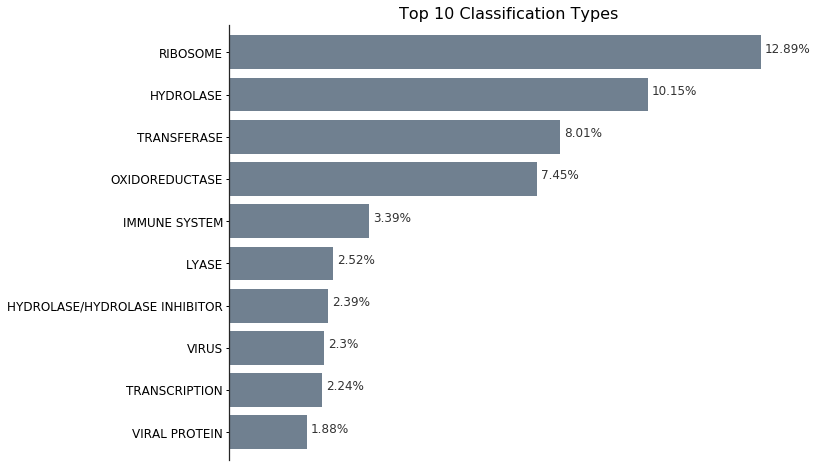
\includegraphics[width=\linewidth]{3.png}
  \caption{Top 10 classification}
  \label{3}
\end{figure}

\subsubsection{Vectorization}
One of the vital stages in our pipeline is converting a sequence of amino acids of data into features that are readable to machine learning models. Here we adopt the Count-Vectorization method that is frequently utilized in NLP problems to vectorize the sequences. Given a sequence of amino acids, it counts the frequency of each amino acid and then output a vector of frequency. However, the drawback of this approach is obvious, it failed to address the connection between adjacent amino acids and only the count of each amino acid will impact the output. In proteins, it is not the individual amino acids that determine the characteristics of the protein. We must also consider the secondary and tertiary structures that are formed via the bonds of amino acids, in other words, the arrangement of amino acids does matter. Hence, we need to take more than one of the continuous amino acids as our frequency counter, or short sequence, in this approach. By increasing this range, we make the kinds of short sequence much greater and hence result in sparser vector. The figure.1 below illustrates the vectorization process. In range size greater than 1, the features would be the count of short sequences like ‘AA, AM, AH’. Our analysis afterwards includes the investigation relationship of this range with the model performance. Figure.\ref{1} illustrates the vectorization process, when we set word size to be 2 in sequence.

\begin{figure*}[h]
  \centering
  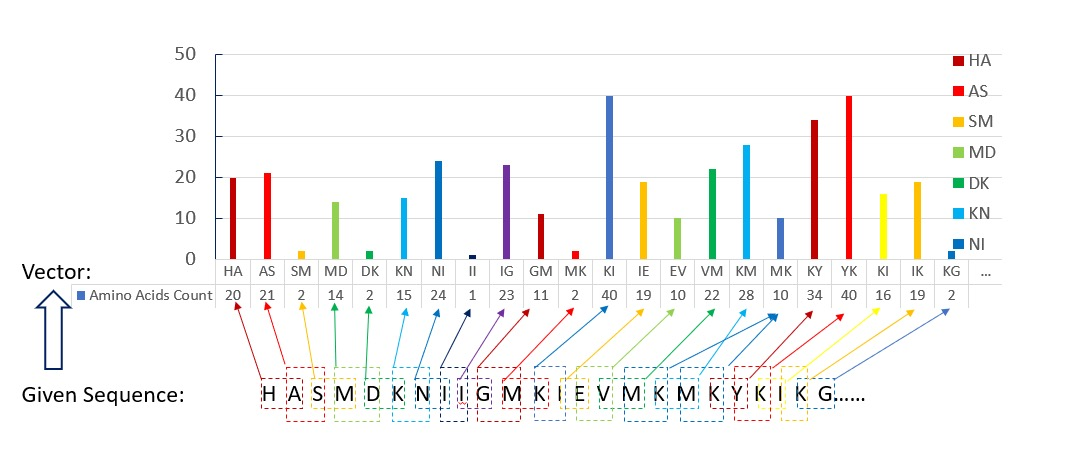
\includegraphics[width=\linewidth]{1.jpeg}
  \caption{Illustration of the vectorization process, word size = 2}
  \label{1}
\end{figure*}

\subsubsection{Correlation}
We also considered other features in the dataset, such as residueCount, resolution, etc.. In order to get a better understanding of the correlations between the physical attributes, we build a Pearson Correlation Matrix. An absolute value closer to 1 represents a stronger correlation between the two factors, further represents a weaker correlation. From the plot below\ref{2} we can tell that these attributes all have fairly small correlation with the classification.

\begin{figure}
  \centering
  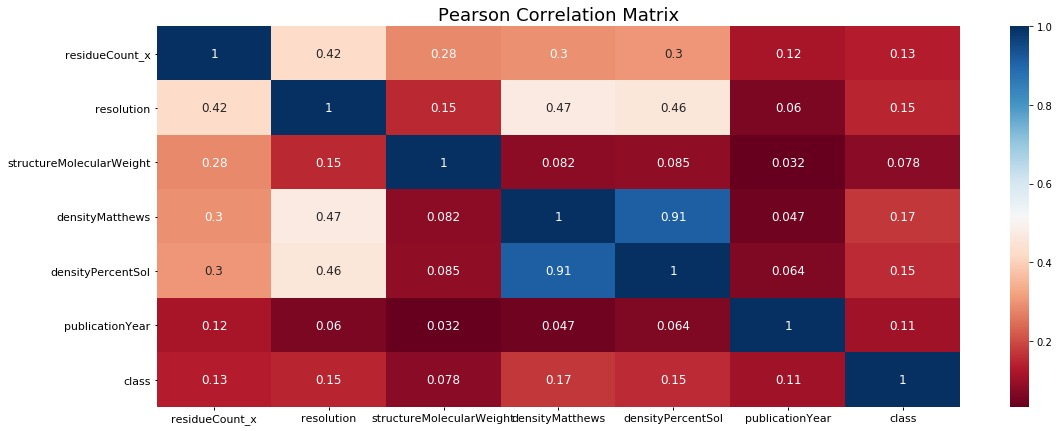
\includegraphics[width=\linewidth]{2.jpeg}
  \caption{Pearson Correlation Matrix for other features in the dataset}
  \label{1}
\end{figure}

\section{Methods}
\subsection{Naive Bayes}
Naive Bayes methods are a set of supervised learning algorithms based on applying Bayes’ theorem with the “naive” assumption of conditional independence between every pair of features given the value of the class variable\cite{patil2013performance}. Bayes’ theorem states the following relationship, given class variable y and dependent feature vector $x_1$ through $x_n$:
\begin{equation}
    P(y \mid x_1, \dots, x_n) = \frac{P(y) P(x_1, \dots x_n \mid y)}{P(x_1, \dots, x_n)}
\end{equation}

Using the naive conditional independence assumption that
\begin{equation}
    P(x_i | y, x_1, \dots, x_{i-1}, x_{i+1}, \dots, x_n) = P(x_i | y),
\end{equation}
for all i, this relationship is simplified to
\begin{equation}
    P(y \mid x_1, \dots, x_n) = \frac{P(y) \prod_{i=1}^{n} P(x_i \mid y)}{P(x_1, \dots, x_n)}
\end{equation}
Since P($x_1$, \dots, $x_n$) is constant given the input, we can use the following classification rule:
\begin{align}
\begin{aligned}
    P(y \mid x_1, \dots, x_n) \propto P(y) \prod_{i=1}^{n} P(x_i \mid y)\\\Downarrow\\\hat{y} = \arg\max_y P(y) \prod_{i=1}^{n} P(x_i \mid y)
\end{aligned}
\end{align}
and we can use Maximum A Posteriori (MAP) estimation to estimate P(y) and P($x_i \mid y$); the former is then the relative frequency of class y in the training set.

\subsection{Adaboost}
The core principle of AdaBoost is to fit a sequence of weak learners (i.e., models that are only slightly better than random guessing, such as small decision trees) on repeatedly modified versions of the data. The predictions from all of them are then combined through a weighted majority vote (or sum) to produce the final prediction. The data modifications at each so-called boosting iteration consist of applying weights $w_1, w_2, …,  w_N$ to each of the training samples.\cite{freund1999short}
An AdaBoost classifier is a meta-estimator that begins by fitting a classifier on the original dataset and then fits additional copies of the classifier on the same dataset but where the weights of incorrectly classified instances are adjusted such that subsequent classifiers focus more on difficult cases.

\subsection{Random Forest}
In random forests, each tree in the ensemble is built from a sample drawn with replacement from the training set. When splitting each node during the construction of a tree, the best split is found either from all input features or a random subset of size\cite{liaw2002classification}.
The purpose of these two sources of randomness is to decrease the variance of the forest estimator. Indeed, individual decision trees typically exhibit high variance and tend to overfit. The injected randomness in forests yield decision trees with somewhat decoupled prediction errors. By taking an average of those predictions, some errors can cancel out. Random forests achieve a reduced variance by combining diverse trees, sometimes at the cost of a slight increase in bias.

\subsection{K-Neighbours}
Neighbors-based classification is a type of instance-based learning or non-generalizing learning: it does not attempt to construct a general internal model, but simply stores instances of the training data. Classification is computed from a simple majority vote of the nearest neighbors of each point: a query point is assigned the data class which has the most representatives within the nearest neighbors of the point\cite{chua2006exploiting}.
The k-neighbors classification is the most commonly used technique. The optimal choice of the value k is highly data-dependent: in general a larger k suppresses the effects of noise, but makes the classification boundaries less distinct.

\section{Result & Conclusion}
Figure.\ref{4} shows the performance of different training model with various size of short amino acids. On the one hand, we found that only the Naive Bayes approach is sensitive to the length of short sequence we used in feature extraction. This is because this method mainly based on the calculation of conditional probability, which take each feature independently. If the size of the short sequence is too small, it may have fewer features than expected, and the features may influence each other, which means the features depend on others. So, the max value may be different with the correct label, and the accuracy becomes lower. As the length becomes longer, the correlation of each feature becomes smaller and the results get better. However, the size of sequence length cannot become too long, which may make lots of redundant features and let the training time becomes much longer than normal.

\begin{figure}[h]
  \centering
  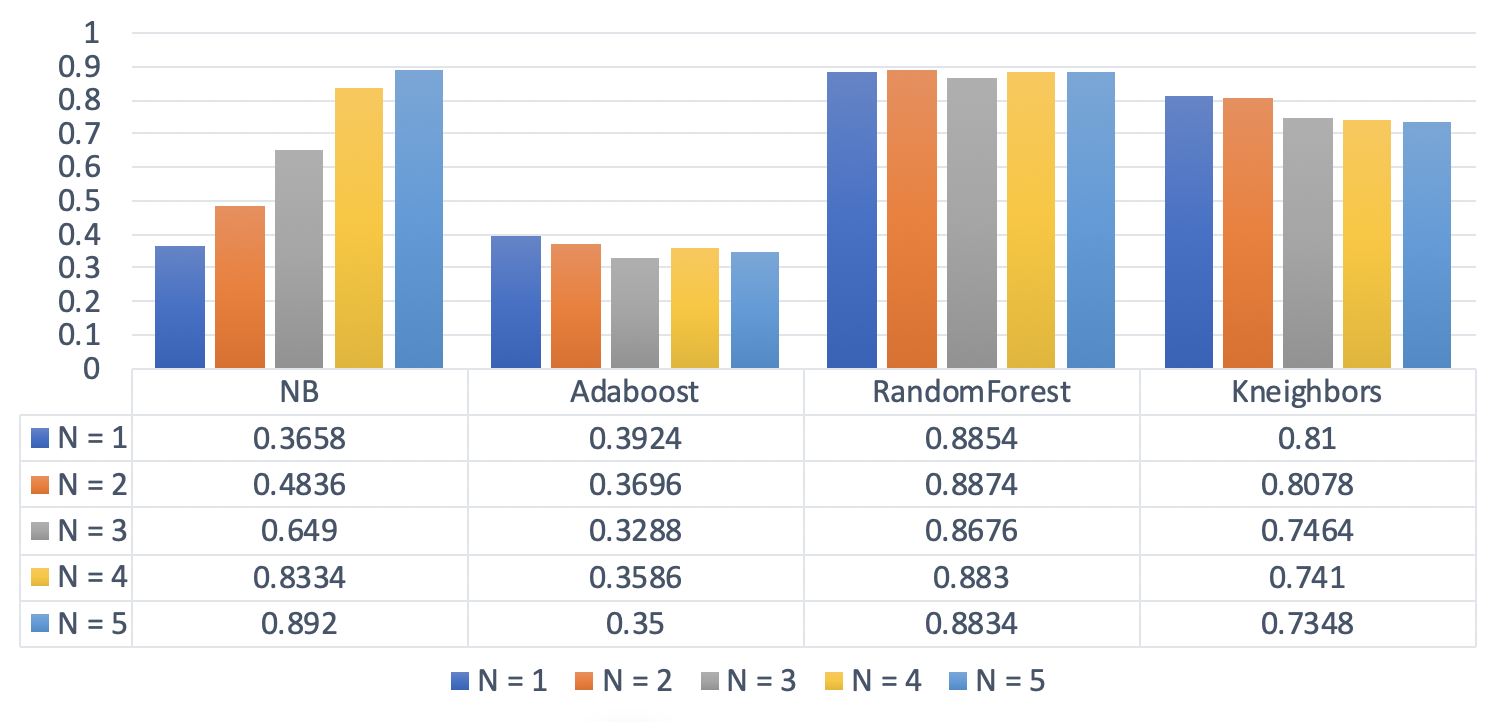
\includegraphics[width=\linewidth]{4.png}
  \caption{Histogram in different training model with various size of amino acids}
  \label{4}
\end{figure}

On the other hand, other approaches don’t depend on this size, which means the training process don’t rely on the independence of each feature. In the future work, we can simply utilize the simple amino acid as a simple feature to train the model.

Therefore, we continue to analysis the Naive Bayes model next. Figure.\ref{5} shows the confusion matrix of Naive Bayes model when setting short sequence range size to be 5. We can observe that the model performs generally the same among the ten categories, there is no significant bias exists as a result of data balancing.

\begin{figure}[h]
  \centering
  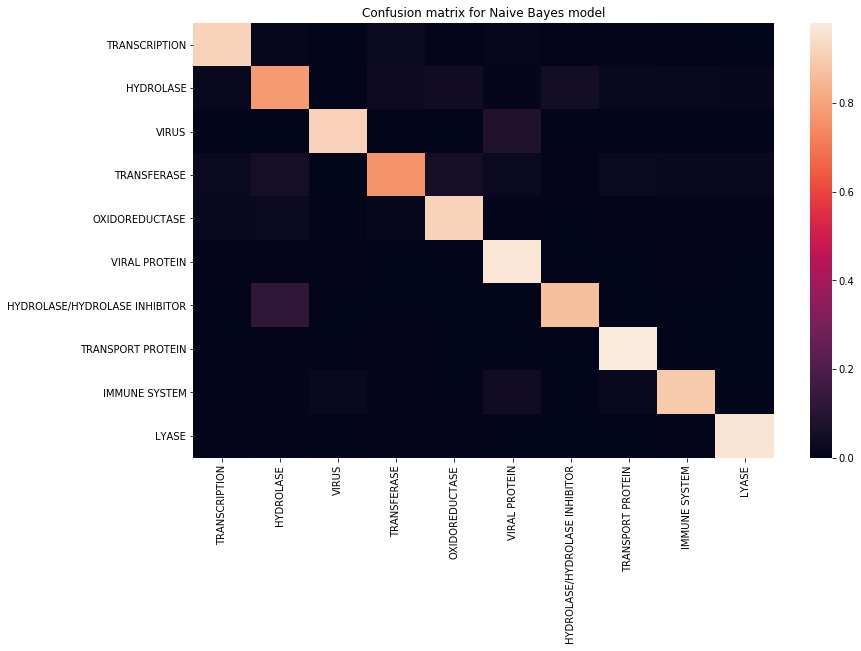
\includegraphics[width=\linewidth]{5.jpeg}
  \caption{The confusion matrix for our best Naïve Bayes model}
  \label{4}
\end{figure}

And Table.\ref{tab} shows the results of our best Naïve Bayes model, we can tell not from the precision rates but also from the recalls that the model behaves generally uniform among the ten categories.

\begin{table*}
  \centering
  \caption{The performance for our best Naïve Bayes based model in each category.}
  \label{tab}
  \begin{tabular}{c|c|c|c|c}
    \toprule
    Class & Precision & Recall & F1-Score & Support \\
    \midrule
    HYDROLASE & 0.74 & 0.78 & 0.76 & 479\\
    TRANSFERASE & 0.9 & 0.76 & 0.82 & 589\\
    VIRAL PROTEIN & 0.81 & 0.97 & 0.88 & 440\\
    TRANSPORT PROTEIN & 0.92 & 0.98 & 0.95 & 469\\
    LYASE & 0.95 & 0.96 & 0.95 & 467\\
    TRANSCRIPTION & 0.91 & 0.92 & 0.91 & 491\\
    VIRUS & 0.96 & 0.91 & 0.94 & 543\\
    OXIDOREDUCTASE & 0.89 & 0.92 & 0.9 & 514\\
    HYDROLASE/HYDROLASE INHIBITOR & 0.94 & 0.87 & 0.9 & 524\\
    IMMUNE SYSTEM & 0.92 & 0.89 & 0.91 & 484\\  
  \bottomrule
\end{tabular}
\end{table*}

\section{Discussion & Future Work}
The drawbacks of our models lie in multiple aspects. Firstly, we failed to address the impacts of amino acids separated by a large distance in the sequence, this may be a main defect to our model assuming that sequence information alone is sufficient to predict the protein function. One of the prospective methods to solve this issue is to use LSTM which could ‘remember’ the information long ago. Secondly, in fact, we cannot assume the sequence alone provides enough features for perfect classification. In real world, proteins generally have a 3-D structure and we cannot know its geometric information based on sequence alone. However, this is an inevitable problem and as a result of our limited biological knowledge, we simply assume that sequence alone is enough. What’s more, one may also wonder why we did not use the other features provided in the dataset as auxiliary information or build ensemble models together with them.

\newpage
\bibliographystyle{ACM-Reference-Format}
\bibliography{sample-base}
\end{document}
\endinput

